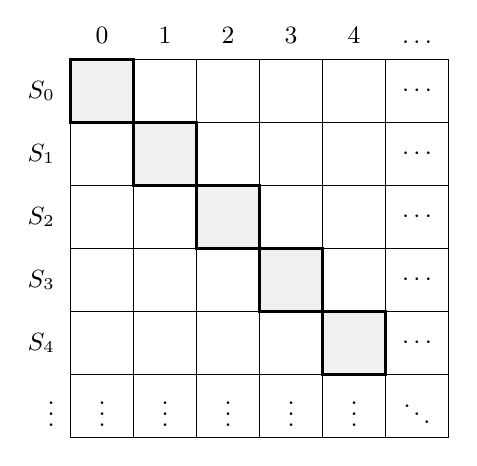
\begin{tikzpicture}[
    every node/.style={font=\small,inner sep=0pt,outer sep=0pt},
    cell/.style ={draw,line width=.4pt,minimum size=8mm,inner sep=0pt},
    tick/.style ={font=\normalsize,green!50!black},
    cross/.style={font=\normalsize,red!70!black}
]

\def\N{4}                      % rows/cols 0…4 are shown explicitly
\pgfmathtruncatemacro\NN{\N+1} % dotted row/column index (=5)

\pgfmathsetseed{15345}         % <- change to get a different random pattern

% ---------------- diagonal box shading (drawn first) ----------------
\foreach \k in {0,...,\N}{
   \fill[black!6] (0.8*\k-0.4,-0.8*\k-0.4) rectangle (0.8*\k+0.4,-0.8*\k+0.4);
}

% ---------------- grid, labels, membership marks ----------------
\foreach \row in {0,...,\NN}{
  \foreach \col in {0,...,\NN}{

      \coordinate (p) at (\col*0.8,-\row*0.8);

      % node name c<row>_<col>
      \node[cell] (c\row_\col) at (p) {};

      % bottom row / rightmost column show dots -----------------
      \ifnum\row=\NN
           \ifnum\col=\NN  \node at (p) {$\ddots$};
           \else           \node at (p) {$\vdots$}; \fi
      \else
           \ifnum\col=\NN  \node at (p) {$\cdots$};
           \else
              % pseudo-random membership mark -------------------
              \pgfmathrandominteger{\rand}{0}{1}
              \ifnum\rand=1
                   \node[tick]  at (p) {\cmark};
              \else \node[cross] at (p) {\xmark}; \fi
           \fi
      \fi
  }
}

% row labels  s_0 … s_N, ⋮
\foreach \row in {0,...,\N}{
   \node[left=2mm] at (c\row_0.west) {$S_{\row}$};
}
\node[left=2mm] at (c\NN_0.west) {$\vdots$};

% column labels 0 … N, …
\foreach \col in {0,...,\N}{
   \node[above=2mm] at (c0_\col.north) {\col};
}
\node[above=2mm] at (c0_\NN.north) {$\dots$};

% bold diagonal boxes
\foreach \k in {0,...,\N}{
   \draw[thick]
         (c\k_\k.north west) rectangle (c\k_\k.south east);
}

\end{tikzpicture}

